\begin{frame}{Perspectives}
Ce qui (n') a (pas) été réussi
Sacrifices faits (système opérationelle)
Problèmes rencontrés (NP-complétude)
Forces et faiblesses du sysème
Pistes à suivre pour une suite éventuelle
Évaluation du système à faire
\end{frame}

\begin{frame}{Perspectives}{Un treillis de concepts en mémoire ?}
\begin{block}{Le contexte}
Un contexte est un triplet $(G,M,I)$ avec
\begin{itemize}
\item $G$ l'ensemble des objets
\item $M$ l'ensemble des attributs
\item $I \subseteq G*M$ l'ensemble des relations
\end{itemize}
On pourrait donc utiliser la mémoire sémantique comme contexte pour la création d'un treillis de concepts.
\end{block}
\end{frame}

\begin{frame}{Perspectives}{Un treillis de concepts en mémoire ?}
\begin{block}{Utile ?}
\begin{itemize}
\item Abstraction supplémentaire
\item Travail sur des ensembles de formes (RPBS)
\end{itemize}
\end{block}
\end{frame}

\begin{frame}{Perspectives}{Un treillis de concepts en mémoire ?}
\begin{block}{Exemple (concret)}
\begin{center}
	\only<1>{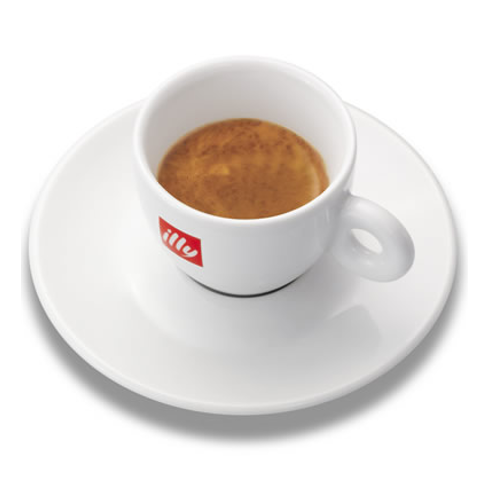
\includegraphics[width=0.2\textwidth]{img/conclusion/espresso_tmp}}
	\only<2->{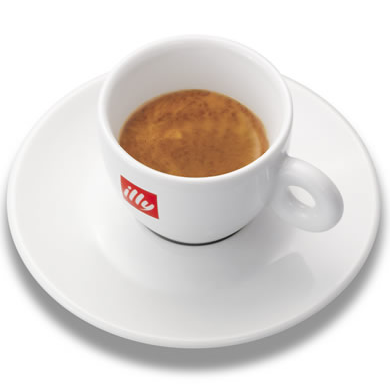
\includegraphics[width=0.2\textwidth]{img/conclusion/espresso}}
	\only<-2>{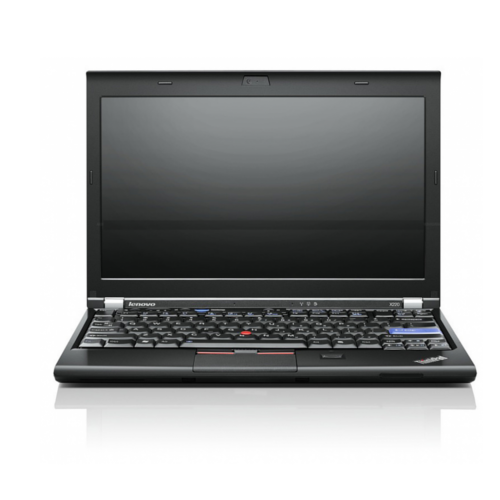
\includegraphics[width=0.2\textwidth]{img/conclusion/ordi_tmp}}
	\only<3->{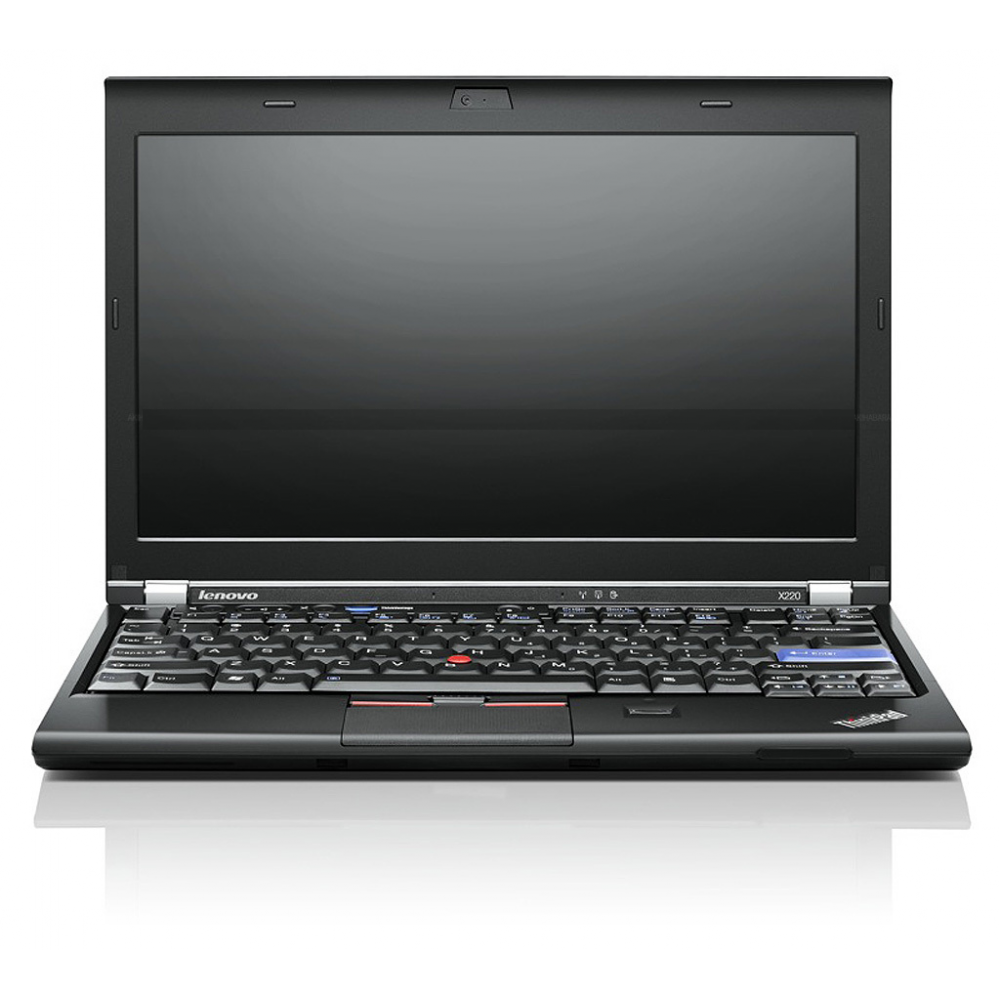
\includegraphics[width=0.2\textwidth]{img/conclusion/ordi}}
\end{center}
\begin{center}
	\only<4>{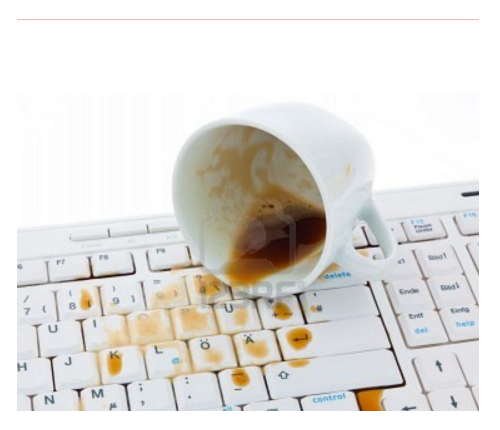
\includegraphics[width=0.3\textwidth]{img/conclusion/cafe_renverse_tmp}}
	\only<5->{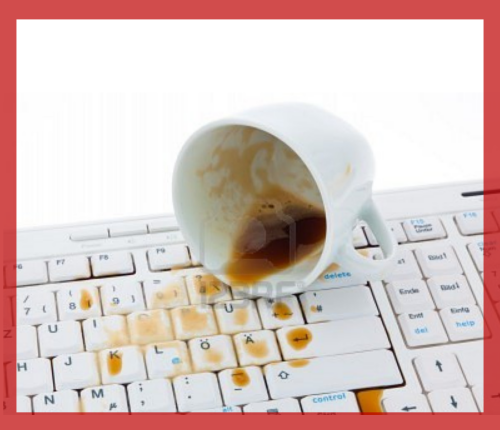
\includegraphics[width=0.3\textwidth]{img/conclusion/cafe_renverse}}
\end{center}
\end{block}
\end{frame}